\section{Kernel and node runtime}\label{sec:arch}

\subsection{Convolution engine}

The kernel is written in C++ for Vitis HLS \cite{amd_ug1399} and processes one window at a time through all layers
of the network on a single convolution engine (Fig.~\ref{fig:kernel}). It stores the activations of a window on chip
in two buffers that alternate between layers, each holding 128 channels of 8 bit values for up to
$13\times13\times13$ sites, so that no intermediate result leaves the FPGA. The engine is weight stationary
\cite{zhang2015optimizing}: for a block of 64 output channels it keeps the 32 bit partial sums of every site on chip;
for each of the 27 kernel offsets and each block of 16 input channels it loads a $64\times16$ block of 8 bit weights
into registers and streams all sites of the window through the engine, one site per clock cycle. At each site the
engine reads the 16 input activations of the neighbour at the kernel offset (zero outside the window, which realizes
the zero padding of the network) and adds 1024 products to the 64 partial sums. After the last offset and input
block, an epilogue pipeline adds the biases and either requantizes and maps the 64 results through the GELU table
(hidden layers) or compares them with the thresholds and writes one bit per output channel (last layer). The weights
of all layers stay in UltraRAM for the lifetime of the kernel and are loaded from HBM once per launch.

\begin{figure}[t]
\centering
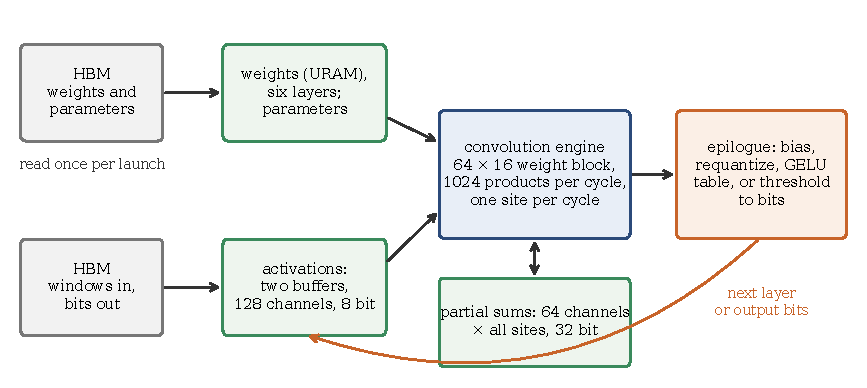
\includegraphics[width=\textwidth]{figures/fig_kernel.pdf}
\caption{Kernel of one instance. Weights and parameters are read from HBM into on chip memories once per launch. For
each window, the convolution engine runs the layers one after the other; activations alternate between two on chip
buffers, and the partial sums of 64 output channels stay on chip for all sites. Each card holds two instances, in SLR1
and SLR2.}\label{fig:kernel}
\end{figure}

\subsection{Epilogue parameters}

A first version read the bias, multiplier and table entry of each of the 64 output channels per cycle from one
parameter memory, at addresses that depend on the layer. HLS partitioned that memory into 144 banks and had not finished
scheduling the epilogue when it was stopped after 7{,}000 seconds. The final kernel copies each layer's biases, multipliers and thresholds
into registers and its activation table into 64 small per channel memories before the sites stream through, so the
epilogue reads every parameter at a fixed lane. With this change C synthesis finishes in about two minutes, every
loop of the engine and epilogue reaches an initiation interval of one, and the estimated maximum clock frequency is
\NumHlsFmax{}~MHz against the 300~MHz target.

\subsection{One bitstream for both networks}

Both networks have 128 hidden channels and differ only in the number of layers, so the layer count is a launch
argument (four or six) and the on chip weight and parameter memories are sized for six layers. The host derives the
layer count from the size of the parameter file; the kernel reads only the weights and parameters of the layers the
host supplies. One bitstream therefore runs the Fast network and the Accurate network.

\subsection{Throughput model}

The work per window is fixed by the network and the window size: $\NumMacsFast$ multiply accumulate operations for the
Fast network at $d=T=9$ and $\NumMacsAcc$ for the Accurate network at $d=T=13$. From the loop structure and the
pipeline depths reported by HLS, a window takes $\NumCyclesFast$ cycles (Fast, $d=9$) or $\NumCyclesAcc$ cycles
(Accurate, $d=13$) on one instance, that is $\NumMacPerCycleFast$ and $\NumMacPerCycleAcc$ useful operations per cycle
out of the 1024 the engine can perform. The difference to the peak comes from the first layer, which has four input
channels on an engine built for 16, the last layer, which has four output channels on an engine built for 64, and the
pipeline fill at each kernel offset. At 300~MHz the model predicts $\NumModelFast$ windows per second per instance for
the Fast network at $d=9$ and $\NumModelAcc$ for the Accurate network at $d=13$.

\subsection{Cards as nodes}

Each card carries two kernel instances, placed in SLR1 and SLR2 because SLR0 also holds the platform's HBM and DMA
logic; each instance has its own two HBM pseudo channels, one for weights and parameters and one for windows and
output bits. As in our multi FPGA statevector work \cite{ali2026multifpga}, every card is a node driven by its own host
process through XRT \cite{amd_xrt}. A process loads the bitstream, copies the weights and parameters to both
instances once, and then keeps two launches per instance in flight so that the transfer of one batch of windows
overlaps the computation of the previous one. For multi card runs all processes finish their setup, wait at a common
start barrier, and report the wall clock interval of their timed loop; the aggregate throughput is the total number of
windows divided by the interval from the first start to the last end. The windows of a batch are independent, so the
nodes exchange no data.
